% Created by tikzDevice version 0.12.6 on 2026-07-04 06:01:30
% !TEX encoding = UTF-8 Unicode
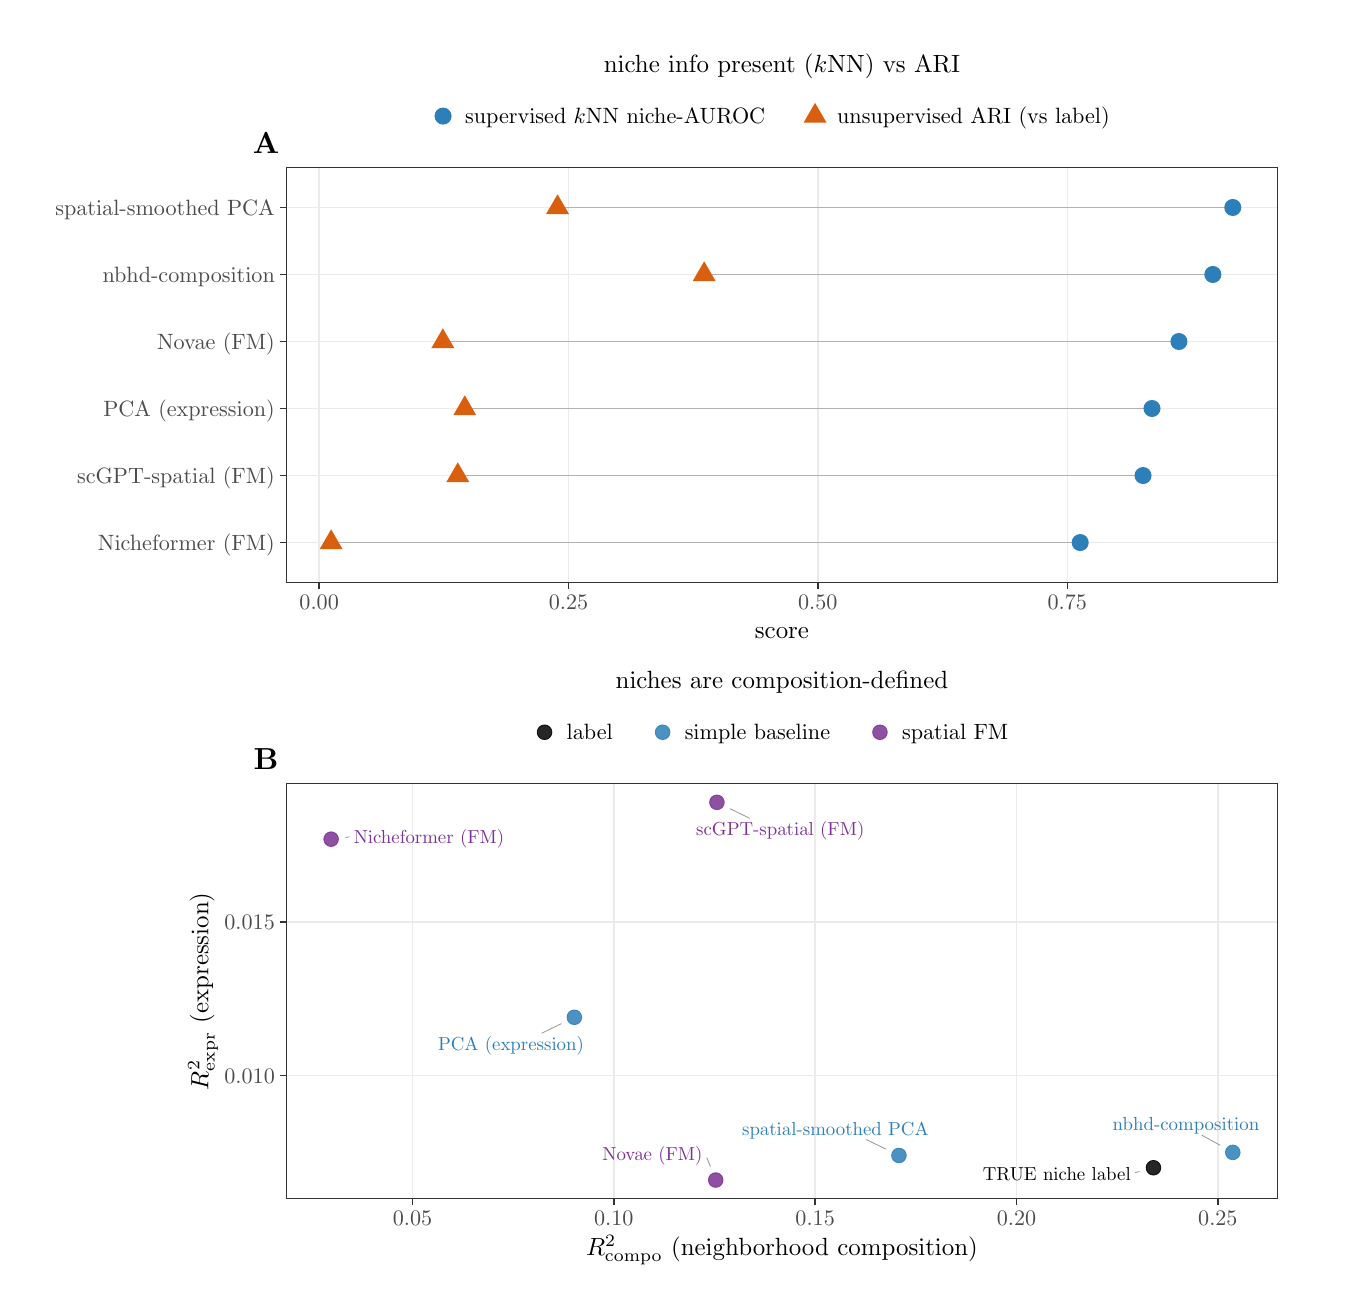
\begin{tikzpicture}[x=1pt,y=1pt]
\definecolor{fillColor}{RGB}{255,255,255}
\path[use as bounding box,fill=fillColor,fill opacity=0.00] (0,0) rectangle (469.75,455.30);
\begin{scope}
\path[clip] (  0.00,  0.00) rectangle (469.75,455.30);
\definecolor{drawColor}{RGB}{255,255,255}
\definecolor{fillColor}{RGB}{255,255,255}

\path[draw=drawColor,line width= 0.5pt,line join=round,line cap=round,fill=fillColor] (  0.00,  0.00) rectangle (469.75,455.30);
\end{scope}
\begin{scope}
\path[clip] (  5.00,227.65) rectangle (460.76,450.30);
\definecolor{drawColor}{RGB}{255,255,255}
\definecolor{fillColor}{RGB}{255,255,255}

\path[draw=drawColor,line width= 0.5pt,line join=round,line cap=round,fill=fillColor] (  5.00,227.65) rectangle (460.76,450.30);
\end{scope}
\begin{scope}
\path[clip] (  5.00,  5.00) rectangle (460.76,227.65);
\definecolor{drawColor}{RGB}{255,255,255}
\definecolor{fillColor}{RGB}{255,255,255}

\path[draw=drawColor,line width= 0.5pt,line join=round,line cap=round,fill=fillColor] (  5.00,  5.00) rectangle (460.76,227.65);
\end{scope}
\begin{scope}
\path[clip] ( 93.36,254.72) rectangle (451.75,404.85);
\definecolor{fillColor}{RGB}{255,255,255}

\path[fill=fillColor] ( 93.36,254.72) rectangle (451.75,404.85);
\definecolor{drawColor}{gray}{0.92}

\path[draw=drawColor,line width= 0.5pt,line join=round] ( 93.36,269.25) --
	(451.75,269.25);

\path[draw=drawColor,line width= 0.5pt,line join=round] ( 93.36,293.46) --
	(451.75,293.46);

\path[draw=drawColor,line width= 0.5pt,line join=round] ( 93.36,317.68) --
	(451.75,317.68);

\path[draw=drawColor,line width= 0.5pt,line join=round] ( 93.36,341.89) --
	(451.75,341.89);

\path[draw=drawColor,line width= 0.5pt,line join=round] ( 93.36,366.11) --
	(451.75,366.11);

\path[draw=drawColor,line width= 0.5pt,line join=round] ( 93.36,390.32) --
	(451.75,390.32);

\path[draw=drawColor,line width= 0.5pt,line join=round] (105.33,254.72) --
	(105.33,404.85);

\path[draw=drawColor,line width= 0.5pt,line join=round] (195.43,254.72) --
	(195.43,404.85);

\path[draw=drawColor,line width= 0.5pt,line join=round] (285.53,254.72) --
	(285.53,404.85);

\path[draw=drawColor,line width= 0.5pt,line join=round] (375.64,254.72) --
	(375.64,404.85);
\definecolor{drawColor}{gray}{0.70}

\path[draw=drawColor,line width= 0.5pt,line join=round] (109.65,269.25) --
	(380.32,269.25);

\path[draw=drawColor,line width= 0.5pt,line join=round] (155.42,293.46) --
	(403.03,293.46);

\path[draw=drawColor,line width= 0.5pt,line join=round] (157.95,317.68) --
	(406.27,317.68);

\path[draw=drawColor,line width= 0.5pt,line join=round] (150.02,341.89) --
	(416.00,341.89);

\path[draw=drawColor,line width= 0.5pt,line join=round] (244.45,366.11) --
	(428.26,366.11);

\path[draw=drawColor,line width= 0.5pt,line join=round] (191.47,390.32) --
	(435.46,390.32);
\definecolor{fillColor}{RGB}{217,95,14}

\path[fill=fillColor] (244.45,370.89) --
	(248.59,363.72) --
	(240.30,363.72) --
	cycle;

\path[fill=fillColor] (157.95,322.46) --
	(162.09,315.28) --
	(153.80,315.28) --
	cycle;

\path[fill=fillColor] (191.47,395.10) --
	(195.61,387.93) --
	(187.32,387.93) --
	cycle;

\path[fill=fillColor] (109.65,274.03) --
	(113.79,266.85) --
	(105.51,266.85) --
	cycle;

\path[fill=fillColor] (150.02,346.67) --
	(154.16,339.50) --
	(145.88,339.50) --
	cycle;

\path[fill=fillColor] (155.42,298.24) --
	(159.57,291.07) --
	(151.28,291.07) --
	cycle;
\definecolor{fillColor}{RGB}{44,127,184}

\path[fill=fillColor] (428.26,366.11) circle (  3.08);

\path[fill=fillColor] (406.27,317.68) circle (  3.08);

\path[fill=fillColor] (435.46,390.32) circle (  3.08);

\path[fill=fillColor] (380.32,269.25) circle (  3.08);

\path[fill=fillColor] (416.00,341.89) circle (  3.08);

\path[fill=fillColor] (403.03,293.46) circle (  3.08);
\definecolor{drawColor}{gray}{0.20}

\path[draw=drawColor,line width= 0.5pt,line join=round,line cap=round] ( 93.36,254.72) rectangle (451.75,404.85);
\end{scope}
\begin{scope}
\path[clip] (  0.00,  0.00) rectangle (469.75,455.30);
\definecolor{drawColor}{gray}{0.30}

\node[text=drawColor,anchor=base east,inner sep=0pt, outer sep=0pt, scale=  0.80] at ( 89.31,266.49) {Nicheformer (FM)};

\node[text=drawColor,anchor=base east,inner sep=0pt, outer sep=0pt, scale=  0.80] at ( 89.31,290.71) {scGPT-spatial (FM)};

\node[text=drawColor,anchor=base east,inner sep=0pt, outer sep=0pt, scale=  0.80] at ( 89.31,314.92) {PCA (expression)};

\node[text=drawColor,anchor=base east,inner sep=0pt, outer sep=0pt, scale=  0.80] at ( 89.31,339.14) {Novae (FM)};

\node[text=drawColor,anchor=base east,inner sep=0pt, outer sep=0pt, scale=  0.80] at ( 89.31,363.35) {nbhd-composition};

\node[text=drawColor,anchor=base east,inner sep=0pt, outer sep=0pt, scale=  0.80] at ( 89.31,387.57) {spatial-smoothed PCA};
\end{scope}
\begin{scope}
\path[clip] (  0.00,  0.00) rectangle (469.75,455.30);
\definecolor{drawColor}{gray}{0.20}

\path[draw=drawColor,line width= 0.5pt,line join=round] ( 91.11,269.25) --
	( 93.36,269.25);

\path[draw=drawColor,line width= 0.5pt,line join=round] ( 91.11,293.46) --
	( 93.36,293.46);

\path[draw=drawColor,line width= 0.5pt,line join=round] ( 91.11,317.68) --
	( 93.36,317.68);

\path[draw=drawColor,line width= 0.5pt,line join=round] ( 91.11,341.89) --
	( 93.36,341.89);

\path[draw=drawColor,line width= 0.5pt,line join=round] ( 91.11,366.11) --
	( 93.36,366.11);

\path[draw=drawColor,line width= 0.5pt,line join=round] ( 91.11,390.32) --
	( 93.36,390.32);
\end{scope}
\begin{scope}
\path[clip] (  0.00,  0.00) rectangle (469.75,455.30);
\definecolor{drawColor}{gray}{0.20}

\path[draw=drawColor,line width= 0.5pt,line join=round] (105.33,252.47) --
	(105.33,254.72);

\path[draw=drawColor,line width= 0.5pt,line join=round] (195.43,252.47) --
	(195.43,254.72);

\path[draw=drawColor,line width= 0.5pt,line join=round] (285.53,252.47) --
	(285.53,254.72);

\path[draw=drawColor,line width= 0.5pt,line join=round] (375.64,252.47) --
	(375.64,254.72);
\end{scope}
\begin{scope}
\path[clip] (  0.00,  0.00) rectangle (469.75,455.30);
\definecolor{drawColor}{gray}{0.30}

\node[text=drawColor,anchor=base,inner sep=0pt, outer sep=0pt, scale=  0.80] at (105.33,245.16) {0.00};

\node[text=drawColor,anchor=base,inner sep=0pt, outer sep=0pt, scale=  0.80] at (195.43,245.16) {0.25};

\node[text=drawColor,anchor=base,inner sep=0pt, outer sep=0pt, scale=  0.80] at (285.53,245.16) {0.50};

\node[text=drawColor,anchor=base,inner sep=0pt, outer sep=0pt, scale=  0.80] at (375.64,245.16) {0.75};
\end{scope}
\begin{scope}
\path[clip] (  0.00,  0.00) rectangle (469.75,455.30);
\definecolor{drawColor}{RGB}{0,0,0}

\node[text=drawColor,anchor=base,inner sep=0pt, outer sep=0pt, scale=  0.90] at (272.56,234.40) {score};
\end{scope}
\begin{scope}
\path[clip] (  0.00,  0.00) rectangle (469.75,455.30);
\definecolor{fillColor}{RGB}{255,255,255}

\path[fill=fillColor] (140.60,413.85) rectangle (404.51,432.85);
\end{scope}
\begin{scope}
\path[clip] (  0.00,  0.00) rectangle (469.75,455.30);
\definecolor{fillColor}{RGB}{255,255,255}

\path[fill=fillColor] (145.10,418.35) rectangle (155.10,428.35);
\definecolor{fillColor}{RGB}{44,127,184}

\path[fill=fillColor] (150.10,423.35) circle (  3.08);
\end{scope}
\begin{scope}
\path[clip] (  0.00,  0.00) rectangle (469.75,455.30);
\definecolor{fillColor}{RGB}{255,255,255}

\path[fill=fillColor] (279.52,418.35) rectangle (289.52,428.35);
\definecolor{fillColor}{RGB}{217,95,14}

\path[fill=fillColor] (284.52,428.13) --
	(288.66,420.96) --
	(280.38,420.96) --
	cycle;
\end{scope}
\begin{scope}
\path[clip] (  0.00,  0.00) rectangle (469.75,455.30);
\definecolor{drawColor}{RGB}{0,0,0}

\node[text=drawColor,anchor=base west,inner sep=0pt, outer sep=0pt, scale=  0.80] at (158.10,420.60) {supervised $k$NN niche-AUROC};
\end{scope}
\begin{scope}
\path[clip] (  0.00,  0.00) rectangle (469.75,455.30);
\definecolor{drawColor}{RGB}{0,0,0}

\node[text=drawColor,anchor=base west,inner sep=0pt, outer sep=0pt, scale=  0.80] at (292.52,420.60) {unsupervised ARI (vs label)};
\end{scope}
\begin{scope}
\path[clip] (  0.00,  0.00) rectangle (469.75,455.30);
\definecolor{drawColor}{RGB}{0,0,0}

\node[text=drawColor,anchor=base,inner sep=0pt, outer sep=0pt, scale=  0.90] at (272.56,439.10) {niche info present ($k$NN) vs ARI};
\end{scope}
\begin{scope}
\path[clip] (  0.00,  0.00) rectangle (469.75,455.30);
\definecolor{drawColor}{RGB}{0,0,0}

\node[text=drawColor,anchor=base,inner sep=0pt, outer sep=0pt, scale=  1.10] at ( 86.19,410.01) {\bfseries A};
\end{scope}
\begin{scope}
\path[clip] ( 93.36, 32.07) rectangle (451.75,182.20);
\definecolor{fillColor}{RGB}{255,255,255}

\path[fill=fillColor] ( 93.36, 32.07) rectangle (451.75,182.20);
\definecolor{drawColor}{gray}{0.92}

\path[draw=drawColor,line width= 0.5pt,line join=round] ( 93.36, 76.62) --
	(451.75, 76.62);

\path[draw=drawColor,line width= 0.5pt,line join=round] ( 93.36,132.10) --
	(451.75,132.10);

\path[draw=drawColor,line width= 0.5pt,line join=round] (139.05, 32.07) --
	(139.05,182.20);

\path[draw=drawColor,line width= 0.5pt,line join=round] (211.80, 32.07) --
	(211.80,182.20);

\path[draw=drawColor,line width= 0.5pt,line join=round] (284.56, 32.07) --
	(284.56,182.20);

\path[draw=drawColor,line width= 0.5pt,line join=round] (357.32, 32.07) --
	(357.32,182.20);

\path[draw=drawColor,line width= 0.5pt,line join=round] (430.08, 32.07) --
	(430.08,182.20);
\definecolor{drawColor}{RGB}{0,0,0}
\definecolor{fillColor}{RGB}{0,0,0}

\path[draw=drawColor,draw opacity=0.85,line width= 0.3pt,line join=round,line cap=round,fill=fillColor,fill opacity=0.85] (406.80, 43.33) circle (  2.65);
\definecolor{drawColor}{RGB}{44,127,184}
\definecolor{fillColor}{RGB}{44,127,184}

\path[draw=drawColor,draw opacity=0.85,line width= 0.3pt,line join=round,line cap=round,fill=fillColor,fill opacity=0.85] (435.46, 48.88) circle (  2.65);

\path[draw=drawColor,draw opacity=0.85,line width= 0.3pt,line join=round,line cap=round,fill=fillColor,fill opacity=0.85] (197.54, 97.70) circle (  2.65);

\path[draw=drawColor,draw opacity=0.85,line width= 0.3pt,line join=round,line cap=round,fill=fillColor,fill opacity=0.85] (314.83, 47.77) circle (  2.65);
\definecolor{drawColor}{RGB}{123,50,148}
\definecolor{fillColor}{RGB}{123,50,148}

\path[draw=drawColor,draw opacity=0.85,line width= 0.3pt,line join=round,line cap=round,fill=fillColor,fill opacity=0.85] (109.65,162.06) circle (  2.65);

\path[draw=drawColor,draw opacity=0.85,line width= 0.3pt,line join=round,line cap=round,fill=fillColor,fill opacity=0.85] (248.62, 38.89) circle (  2.65);

\path[draw=drawColor,draw opacity=0.85,line width= 0.3pt,line join=round,line cap=round,fill=fillColor,fill opacity=0.85] (249.06,175.38) circle (  2.65);
\definecolor{drawColor}{gray}{0.60}

\path[draw=drawColor,line width= 0.3pt,line join=round,line cap=round] (400.24, 41.57) -- (401.69, 41.96);

\path[draw=drawColor,line width= 0.3pt,line join=round,line cap=round] (424.27, 55.13) -- (430.85, 51.46);

\path[draw=drawColor,line width= 0.3pt,line join=round,line cap=round] (185.79, 91.96) -- (192.79, 95.38);

\path[draw=drawColor,line width= 0.3pt,line join=round,line cap=round] (303.04, 53.52) -- (310.08, 50.09);

\path[draw=drawColor,line width= 0.3pt,line join=round,line cap=round] (116.22,162.88) -- (114.90,162.71);

\path[draw=drawColor,line width= 0.3pt,line join=round,line cap=round] (245.43, 46.95) -- (246.68, 43.81);

\path[draw=drawColor,line width= 0.3pt,line join=round,line cap=round] (260.81,169.64) -- (253.81,173.06);
\definecolor{drawColor}{RGB}{0,0,0}

\node[text=drawColor,anchor=base,inner sep=0pt, outer sep=0pt, scale=  0.68] at (371.89, 38.69) {TRUE niche label};
\definecolor{drawColor}{RGB}{44,127,184}

\node[text=drawColor,anchor=base,inner sep=0pt, outer sep=0pt, scale=  0.68] at (418.55, 56.64) {nbhd-composition};

\node[text=drawColor,anchor=base,inner sep=0pt, outer sep=0pt, scale=  0.68] at (174.65, 85.75) {PCA (expression)};

\node[text=drawColor,anchor=base,inner sep=0pt, outer sep=0pt, scale=  0.68] at (291.87, 55.03) {spatial-smoothed PCA};
\definecolor{drawColor}{RGB}{123,50,148}

\node[text=drawColor,anchor=base,inner sep=0pt, outer sep=0pt, scale=  0.68] at (145.01,160.57) {Nicheformer (FM)};

\node[text=drawColor,anchor=base,inner sep=0pt, outer sep=0pt, scale=  0.68] at (225.77, 46.11) {Novae (FM)};

\node[text=drawColor,anchor=base,inner sep=0pt, outer sep=0pt, scale=  0.68] at (271.95,163.43) {scGPT-spatial (FM)};
\definecolor{drawColor}{gray}{0.20}

\path[draw=drawColor,line width= 0.5pt,line join=round,line cap=round] ( 93.36, 32.07) rectangle (451.75,182.20);
\end{scope}
\begin{scope}
\path[clip] (  0.00,  0.00) rectangle (469.75,455.30);
\definecolor{drawColor}{gray}{0.20}

\path[draw=drawColor,line width= 0.5pt,line join=round] (139.05, 29.82) --
	(139.05, 32.07);

\path[draw=drawColor,line width= 0.5pt,line join=round] (211.80, 29.82) --
	(211.80, 32.07);

\path[draw=drawColor,line width= 0.5pt,line join=round] (284.56, 29.82) --
	(284.56, 32.07);

\path[draw=drawColor,line width= 0.5pt,line join=round] (357.32, 29.82) --
	(357.32, 32.07);

\path[draw=drawColor,line width= 0.5pt,line join=round] (430.08, 29.82) --
	(430.08, 32.07);
\end{scope}
\begin{scope}
\path[clip] (  0.00,  0.00) rectangle (469.75,455.30);
\definecolor{drawColor}{gray}{0.30}

\node[text=drawColor,anchor=base,inner sep=0pt, outer sep=0pt, scale=  0.80] at (139.05, 22.51) {0.05};

\node[text=drawColor,anchor=base,inner sep=0pt, outer sep=0pt, scale=  0.80] at (211.80, 22.51) {0.10};

\node[text=drawColor,anchor=base,inner sep=0pt, outer sep=0pt, scale=  0.80] at (284.56, 22.51) {0.15};

\node[text=drawColor,anchor=base,inner sep=0pt, outer sep=0pt, scale=  0.80] at (357.32, 22.51) {0.20};

\node[text=drawColor,anchor=base,inner sep=0pt, outer sep=0pt, scale=  0.80] at (430.08, 22.51) {0.25};
\end{scope}
\begin{scope}
\path[clip] (  0.00,  0.00) rectangle (469.75,455.30);
\definecolor{drawColor}{RGB}{0,0,0}

\node[text=drawColor,anchor=base,inner sep=0pt, outer sep=0pt, scale=  0.90] at (272.56, 11.75) {$R^2_{\mathrm{compo}}$ (neighborhood composition)};
\end{scope}
\begin{scope}
\path[clip] (  0.00,  0.00) rectangle (469.75,455.30);
\definecolor{drawColor}{gray}{0.30}

\node[text=drawColor,anchor=base east,inner sep=0pt, outer sep=0pt, scale=  0.80] at ( 89.31, 73.86) {0.010};

\node[text=drawColor,anchor=base east,inner sep=0pt, outer sep=0pt, scale=  0.80] at ( 89.31,129.34) {0.015};
\end{scope}
\begin{scope}
\path[clip] (  0.00,  0.00) rectangle (469.75,455.30);
\definecolor{drawColor}{gray}{0.20}

\path[draw=drawColor,line width= 0.5pt,line join=round] ( 91.11, 76.62) --
	( 93.36, 76.62);

\path[draw=drawColor,line width= 0.5pt,line join=round] ( 91.11,132.10) --
	( 93.36,132.10);
\end{scope}
\begin{scope}
\path[clip] (  0.00,  0.00) rectangle (469.75,455.30);
\definecolor{drawColor}{RGB}{0,0,0}

\node[text=drawColor,rotate= 90.00,anchor=base,inner sep=0pt, outer sep=0pt, scale=  0.90] at ( 65.34,107.13) {$R^2_{\mathrm{expr}}$ (expression)};
\end{scope}
\begin{scope}
\path[clip] (  0.00,  0.00) rectangle (469.75,455.30);
\definecolor{fillColor}{RGB}{255,255,255}

\path[fill=fillColor] (177.27,191.20) rectangle (367.85,210.20);
\end{scope}
\begin{scope}
\path[clip] (  0.00,  0.00) rectangle (469.75,455.30);
\definecolor{fillColor}{RGB}{255,255,255}

\path[fill=fillColor] (181.77,195.70) rectangle (191.77,205.70);
\definecolor{drawColor}{RGB}{0,0,0}
\definecolor{fillColor}{RGB}{0,0,0}

\path[draw=drawColor,draw opacity=0.85,line width= 0.3pt,line join=round,line cap=round,fill=fillColor,fill opacity=0.85] (186.77,200.70) circle (  2.65);
\end{scope}
\begin{scope}
\path[clip] (  0.00,  0.00) rectangle (469.75,455.30);
\definecolor{fillColor}{RGB}{255,255,255}

\path[fill=fillColor] (224.44,195.70) rectangle (234.44,205.70);
\definecolor{drawColor}{RGB}{44,127,184}
\definecolor{fillColor}{RGB}{44,127,184}

\path[draw=drawColor,draw opacity=0.85,line width= 0.3pt,line join=round,line cap=round,fill=fillColor,fill opacity=0.85] (229.44,200.70) circle (  2.65);
\end{scope}
\begin{scope}
\path[clip] (  0.00,  0.00) rectangle (469.75,455.30);
\definecolor{fillColor}{RGB}{255,255,255}

\path[fill=fillColor] (302.97,195.70) rectangle (312.97,205.70);
\definecolor{drawColor}{RGB}{123,50,148}
\definecolor{fillColor}{RGB}{123,50,148}

\path[draw=drawColor,draw opacity=0.85,line width= 0.3pt,line join=round,line cap=round,fill=fillColor,fill opacity=0.85] (307.97,200.70) circle (  2.65);
\end{scope}
\begin{scope}
\path[clip] (  0.00,  0.00) rectangle (469.75,455.30);
\definecolor{drawColor}{RGB}{0,0,0}

\node[text=drawColor,anchor=base west,inner sep=0pt, outer sep=0pt, scale=  0.80] at (194.77,197.95) {label};
\end{scope}
\begin{scope}
\path[clip] (  0.00,  0.00) rectangle (469.75,455.30);
\definecolor{drawColor}{RGB}{0,0,0}

\node[text=drawColor,anchor=base west,inner sep=0pt, outer sep=0pt, scale=  0.80] at (237.44,197.95) {simple baseline};
\end{scope}
\begin{scope}
\path[clip] (  0.00,  0.00) rectangle (469.75,455.30);
\definecolor{drawColor}{RGB}{0,0,0}

\node[text=drawColor,anchor=base west,inner sep=0pt, outer sep=0pt, scale=  0.80] at (315.97,197.95) {spatial FM};
\end{scope}
\begin{scope}
\path[clip] (  0.00,  0.00) rectangle (469.75,455.30);
\definecolor{drawColor}{RGB}{0,0,0}

\node[text=drawColor,anchor=base,inner sep=0pt, outer sep=0pt, scale=  0.90] at (272.56,216.45) {niches are composition-defined};
\end{scope}
\begin{scope}
\path[clip] (  0.00,  0.00) rectangle (469.75,455.30);
\definecolor{drawColor}{RGB}{0,0,0}

\node[text=drawColor,anchor=base,inner sep=0pt, outer sep=0pt, scale=  1.10] at ( 86.19,187.36) {\bfseries B};
\end{scope}
\end{tikzpicture}
